\documentclass[a4paper,twoside]{article}
\usepackage[T1]{fontenc}
\usepackage[bahasa]{babel}
\usepackage{graphicx}
\usepackage{graphics}
\usepackage{float}
\usepackage[cm]{fullpage}
\pagestyle{myheadings}
\usepackage{etoolbox}
\usepackage{setspace} 
\usepackage{lipsum} 
\setlength{\headsep}{30pt}
\usepackage[inner=2cm,outer=2.5cm,top=2.5cm,bottom=2cm]{geometry} %margin
% \pagestyle{empty}

\makeatletter
\renewcommand{\@maketitle} {\begin{center} {\LARGE \textbf{ \textsc{\@title}} \par} \bigskip {\large \textbf{\textsc{\@author}} }\end{center} }
\renewcommand{\thispagestyle}[1]{}
\markright{\textbf{\textsc{Laporan Perkembangan Pengerjaan Skripsi\textemdash Sem. Ganjil 2019/2020}}}

\onehalfspacing
 
\begin{document}

\title{\@judultopik}
\author{\nama \textendash \@npm} 

%ISILAH DATA BERIKUT INI:
\newcommand{\nama}{Chris Eldon}
\newcommand{\@npm}{2016730073}
\newcommand{\tanggal}{19/11/2019} %Tanggal pembuatan dokumen
\newcommand{\@judultopik}{Privacy Preserving Data Mining dengan Metode Randomization} % Judul/topik anda
\newcommand{\kodetopik}{MTA4703}
\newcommand{\jumpemb}{1} % Jumlah pembimbing, 1 atau 2
\newcommand{\pembA}{Mariskha Tri Adithia, P.D.Eng}
\newcommand{\pembB}{-}
\newcommand{\semesterPertama}{47 - Ganjil 19/20} % semester pertama kali topik diambil, angka 1 dimulai dari sem Ganjil 96/97
\newcommand{\lamaSkripsi}{1} % Jumlah semester untuk mengerjakan skripsi s.d. dokumen ini dibuat
\newcommand{\kulPertama}{Skripsi 1} % Kuliah dimana topik ini diambil pertama kali
\newcommand{\tipePR}{B} % tipe progress report :
% A : dokumen pendukung untuk pengambilan ke-2 di Skripsi 1
% B : dokumen untuk reviewer pada presentasi dan review Skripsi 1
% C : dokumen pendukung untuk pengambilan ke-2 di Skripsi 2

% Dokumen hasil template ini harus dicetak bolak-balik !!!!

\maketitle

\pagenumbering{arabic}

\section{Data Skripsi} %TIDAK PERLU MENGUBAH BAGIAN INI !!!
Pembimbing utama/tunggal: {\bf \pembA}\\
Pembimbing pendamping: {\bf \pembB}\\
Kode Topik : {\bf \kodetopik}\\
Topik ini sudah dikerjakan selama : {\bf \lamaSkripsi} semester\\
Pengambilan pertama kali topik ini pada : Semester {\bf \semesterPertama} \\
Pengambilan pertama kali topik ini di kuliah : {\bf \kulPertama} \\
Tipe Laporan : {\bf \tipePR} -
\ifdefstring{\tipePR}{A}{
			Dokumen pendukung untuk {\BF pengambilan ke-2 di Skripsi 1} }
		{
		\ifdefstring{\tipePR}{B} {
				Dokumen untuk reviewer pada presentasi dan {\bf review Skripsi 1}}
			{	Dokumen pendukung untuk {\bf pengambilan ke-2 di Skripsi 2}}
		}
		
\section{Latar Belakang}
Dengan semakin banyaknya penambangan data yang dilakukan dan data yang digunakan juga semakin banyak, semakin banyak juga privasi di dalam data tersebut yang tersebar kepada pihak yang melakukan penambangan data. Data privasi tersebut dapat tersebar kepada pihak yang tidak bertanggung jawab dan disalahgunakan. Oleh karena itu perlu adanya suatu cara untuk mencegah privasi tersebar pada proses penambangan data, menjaga privasi pada data tersebut. Istilah untuk hal tersebut adalah \textit{privacy preserving data mining}.

Salah satu cara untuk melakukan \textit{privacy preserving data mining} adalah dengan melakukan modifikasi data yang ada sebelum diberikan kepada pihak lain. Ada macam-macam teknik dan algoritma yang bertujuan modifikasi data untuk \textit{privacy preserving data mining} yang bisa dibagi menjadi dua jenis yaitu \textit{Perturbation Approach} dan \textit{Anonymization Approach}. \textit{Perturbation Approach} adalah pendekatan untuk \textit{privacy preserving data mining} dengan cara mengacaukan data yang ada, tetapi hasil data yang dikacaukan masih tetap bisa ditambang. \textit{Perturbation Approach} bisa dibagi menjadi dua jenis yaitu \textit{Value-based Perturbation Techniques} dan \textit{Multi-Dimensional Perturbation}.

\textit{Value-based Perturbation Techniques} adalah teknik yang bekerja dengan cara menyisipkan \textit{random noise} pada data. Sedangkan terdapat dua jenis teknik \textit{Multi-Dimensional Perturbation} yaitu \textit{Data mining Task-based Perturbation} dan \textit{Dimension Reduction-based Perturbation}. \textit{Data mining Task-based Perturbation} adalah teknik yang bekerja dengan cara modifikasi data sehingga properti yang bertahan pada data yang telah dimodifikasi spesifik hanya properti yang digunakan oleh suatu teknik penambangan data tertentu. Sedangkan \textit{Dimension Reduction-based Perturbation} adalah teknik yang bekerja dengan cara modifikasi data sekaligus mengurangi dimensi dari data asli.

\begin{figure}
	\centering
	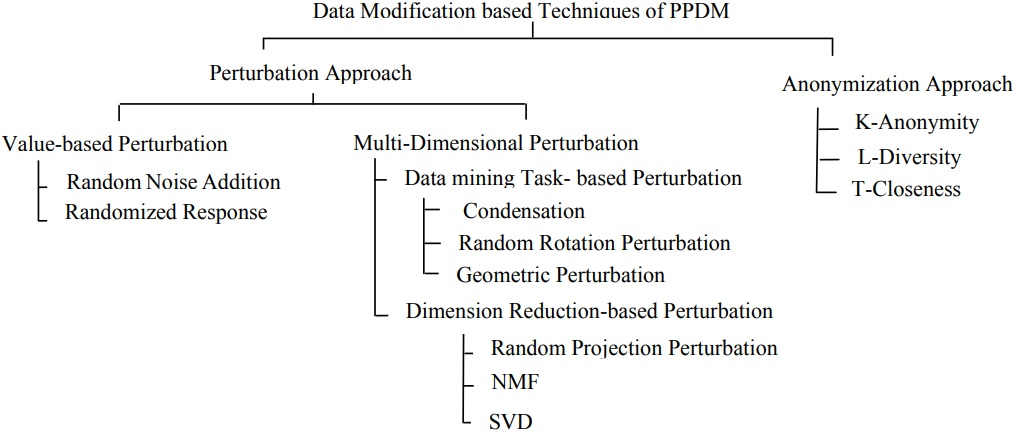
\includegraphics[scale=0.56]{ppdm}
	\caption{Berbagai macam teknik modifikasi data untuk \textit{privacy preserving data mining}}
	\label{fig:ppdm}
\end{figure}

Dari berbagai macam teknik modifikasi data untuk \textit{privacy preserving data mining} yang dapat dilihat pada Gambar \ref{fig:ppdm}, terdapat empat teknik yang menggunakan metode \textit{Randomization} yaitu \textit{Random Noise Addition}, \textit{Randomized Response}, \textit{Random Rotation Perturbation}, dan \textit{Random Projection Perturbation}.

Pada penelitian ini, akan dibuat sebuah perangkat lunak yang dapat memproses data yang akan ditambang menjadi data yang telah dimodifikasi dengan metode \textit{Randomization} sehingga tidak mengandung privasi, tetapi masih dapat ditambang. Dari berbagai macam teknik dengan metode \textit{Randomization} yang ada, dipilih dua buah teknik yaitu \textit{Random Rotation Perturbation} dan \textit{Random Projection Perturbation} untuk diimplementasikan pada perangkat lunak serta membandingkan hasil dari kedua teknik tersebut.

\section{Rumusan Masalah}
Berdasarkan latar belakang, rumusan masalah pada penelitian ini adalah sebagai berikut.
\begin{enumerate}
	\item Bagaimana cara kerja dari teknik \textit{Random Rotation Perturbation} dan \textit{Random Projection Perturbation} untuk \textit{privacy preserving data mining}?
	\item Bagaimana implementasi dari teknik \textit{Random Rotation Perturbation} dan \textit{Random Projection Perturbation} pada perangkat lunak?
	\item Bagaimana perbandingan antara hasil dari teknik \textit{Random Rotation Perturbation} dan \textit{Random Projection Perturbation}?
\end{enumerate}

\section{Tujuan}
Berdasarkan rumusan masalah, maka tujuan dari penilitian ini adalah sebagai berikut.
\begin{enumerate}
	\item Mempelajari cara kerja dari teknik \textit{Random Rotation Perturbation} dan \textit{Random Projection Perturbation} untuk \textit{privacy preserving data mining}
	\item Mengimplementasikan teknik \textit{Random Rotation Perturbation} dan \textit{Random Projection Perturbation} pada perangkat lunak
	\item Melakukan analisis dan pengujian untuk membandingkan dan mengukur hasil dari teknik \textit{Random Rotation Perturbation} dan \textit{Random Projection Perturbation}
\end{enumerate}

\section{Detail Perkembangan Pengerjaan Skripsi}
Detail bagian pekerjaan skripsi sesuai dengan rencana kerja/laporan perkembangan terkahir :
	\begin{enumerate}
		\item \textbf{Melakukan studi literatur mengenai dasar-dasar privasi data}\\
		{\bf Status :} Ada sejak rencana kerja skripsi.\\
		{\bf Hasil :} Pada umumnya sebuah data bisa dikatakan privasi apabila data tersebut dapat dikaitkan dengan identitas seseorang. Tetapi setiap orang memiliki kepentingan privasi yang berbeda-beda sehingga definisi dari privasi sulit untuk dijelaskan secara eksak. Oleh karena itu, perlu adanya konsep privasi yang dapat menjadi acuan untuk menentukan data seperti apa yang termasuk privasi atau bukan.

		Dalam mendefinisikan privasi, sulit untuk mendapatkan definisi yang tepat untuk privasi karena setiap individu memiliki kepentingan yang berbeda-beda sehingga privasi pada setiap individu dapat berbeda-beda juga. Beberapa definisi privasi telah dikemukakan dan definisi tersebut bermacam-macam berdasarkan konteks, budaya, dan lingkungan.~\cite{stanleyosmar:04:standardppdm} Menurut Warren dan Brandeis pada papernya, mereka mendefinisikan privasi sebagai “\textit{the right to be alone.}”, hak untuk menyendiri. Lalu pada papernya, Westin mendefinisikan privasi sebagai “\textit{the desire of people to choose freely under what circumstances and to what extent they will expose themselves, their attitude, and their behavior to others}”, keinginan orang untuk memilih secara bebas dalam segala situasi dan dalam hal mengemukakan diri mereka, sikap mereka, dan tingkah laku mereka pada orang lain. Schoeman mendefinisikan privasi sebagai “\textit{the right to determine what (personal) information is communicated to others}”, hak untuk menentukan informasi pribadi apa saja yang dikomunikasikan kepada yang lain, atau “\textit{the control an individual has over information about himself or herself.}”, kendali seorang individu terhadap informasi tentang dirinya sendiri. Lalu baru-baru ini, Garfinkel menyatakan bahwa “\textit{privacy is about self-possession, autonomy, and integrity.}”, privasi adalah tentang penguasaan diri sendiri, otonomi, dan integritas. Di samping itu, Rosenberg berpendapat bahwa privasi sebenarnya bukan sebuah hak tetapi sebuah rasa: “\textit{If privacy is in the end a matter of individual taste, then seeking a moral foundation for it -- beyond its role in making social institutions possible that we happen to prize -- will be no more fruitful than seeking a moral foundation for the taste for truffles.}”, intinya setiap orang memiliki perhatian yang berbeda-beda terhadap privasi mereka sendiri sehingga hal tersebut tergantung apa yang dirasakan oleh setiap individu.

		Dari definisi-definisi privasi yang telah disebutkan di atas, dapat disimpulkan bahwa privasi dilihat sebagai konsep sosial dan budaya.~\cite{stanleyosmar:04:standardppdm} Konsep privasi pada suatu lingkungan dapat berbeda dari lingkungan lainnya dan hal ini menyebabkan sulitnya menentukan apakah sebuah data termasuk privasi atau bukan. Oleh karena itu, perlu adanya sebuah standar privasi untuk menentukan data mana yang dapat disebut sebuah privasi. Organisasi National Institute of Standards and Technology dari Amerika Serikat, membuat standar mereka sendiri untuk menentukan informasi seperti apa yang dapat disebut sebagai privasi. Mereka mengemukakan konsep \textit{Personally Identifiable Information} sebagai informasi yang dapat dikatakan personal untuk setiap individu.
		
		\item \textbf{Melakukan analisis pada hasil survei terhadap pergerakan pengunjung di museum dan membuat rancangan denah di komputer yang dilengkapi dengan penghalang dan objek di museum.}\\
		{\bf Status :} Ada sejak rencana kerja skripsi.\\
		{\bf Hasil :}

		\item \textbf{Melakukan studi literatur mengenai sifat kolektif suatu kerumunan, teknik {\it social force model} dan teknik {\it flow tiles}}\\
		{\bf Status :} Ada sejak rencana kerja skripsi.\\
		{\bf Hasil :}

		\item \textbf{Mempelajari bahasa pemrograman C++ dan cara menggunakan framework OpenSteer}\\
		{\bf Status :} Ada sejak rencana kerja skripsi.\\
		{\bf Hasil :}

		\item \textbf{Merancang pergerakan kerumunan di dalam museum menggunakan teknik {\it social force model} dan {\it flow tiles} serta menggunakan teknik lainnya seperti konsep pathway dan waypoints. Selain itu, dirancang pula adanya waktu tunggu (pada saat pengunjung melihat objek di museum) dan cara pembuatan jalur bagi setiap individu pengunjung}\\
		{\bf Status :} Ada sejak rencana kerja skripsi.\\
		{\bf Hasil :}

		\item \textbf{Melakukan analisa dan merancang struktur data yang cocok untuk menyimpan penghalang (obstacle)}\\
		{\bf Status :} dihapuskan/tidak dikerjakan \\
		{\bf Hasil :} berdasarkan analisis singkat, tidak dilakukan analisis lebih jauh karena tidak diperlukan struktur data baru, karena sudah disediakan oleh OpenSteer versi terbaru

		\item \textbf{Mengimplementasikan keseluruhan algoritma dan struktur data yang dirancang, dengan menggunakan framework OpenSteer} \\
		{\bf Status :} Ada sejak rencana kerja skripsi.\\
		{\bf Hasil :}

		\item \textbf{Melakukan pengujian (dan eksperimen) yang melibatkan responde untuk menilai hasil simulasi secara kualitatif}\\
		{\bf Status :} Ada sejak rencana kerja skripsi.\\
		{\bf Hasil :}

		\item \textbf{Menulis dokumen skripsi}\\
		{\bf Status :} Ada sejak rencana kerja skripsi.\\
		{\bf Hasil :} \lipsum[1]
		
		\item \textbf{Mempelajari cara menggunakan fitur manipulasi obstacle yang disediakan oleh framework Opensteer versi terbaru}\\
		{\bf Status :} baru ditambahkan pada semester ini\\
		{\bf Hasil :} baru direncanakan karena framework Opensteer versi paling akhir baru selesai diinstall dan dilihat-lihat bagian contoh-contoh simulasinya
		

	\end{enumerate}

\section{Pencapaian Rencana Kerja}
Langkah-langkah kerja yang berhasil diselesaikan dalam Skripsi 1 ini adalah sebagai berikut:
\begin{enumerate}
	\item Mempelajari dasar-dasar privasi data
	\item Mempelajari teknik \textit{Random Noise Addition} dan \textit{Random Rotation Perturbation} untuk \textit{privacy preserving data mining}
	\item Mempelajari teknik penambangan data yang akan digunakan
	\item Melakukan analisis terhadap teknik <<TODO>> dan \textit{Random Rotation Perturbation} serta bagaimana penerapannya dengan teknik penambangan data yang akan digunakan
	\item Menulis dokumen skripsi
\end{enumerate}



\section{Kendala yang Dihadapi}
%TULISKAN BAGIAN INI JIKA DOKUMEN ANDA TIPE A ATAU C
Kendala - kendala yang dihadapi selama mengerjakan skripsi :
\begin{itemize}
	\item Terlalu banyak melakukan prokratinasi
	\item Terlalu banyak godaan berupa hiburan (game, film, dll)
	\item Skripsi diambil bersamaan dengan kuliah ASD karena selama 5 semester pertama kuliah tersebut sangat dihindari dan tidak diambil, dan selama 4 semester terakhir kuliah tersebut selalu mendapat nilai E
	\item Mengalami kesulitan pada saat sudah mulai membuat program komputer karena selama ini selalu dibantu teman
\end{itemize}

\vspace{1cm}
\centering Bandung, \tanggal\\
\vspace{2cm} \nama \\ 
\vspace{1cm}

Menyetujui, \\
\ifdefstring{\jumpemb}{2}{
\vspace{1.5cm}
\begin{centering} Menyetujui,\\ \end{centering} \vspace{0.75cm}
\begin{minipage}[b]{0.45\linewidth}
% \centering Bandung, \makebox[0.5cm]{\hrulefill}/\makebox[0.5cm]{\hrulefill}/2013 \\
\vspace{2cm} Nama: \pembA \\ Pembimbing Utama
\end{minipage} \hspace{0.5cm}
\begin{minipage}[b]{0.45\linewidth}
% \centering Bandung, \makebox[0.5cm]{\hrulefill}/\makebox[0.5cm]{\hrulefill}/2013\\
\vspace{2cm} Nama: \pembB \\ Pembimbing Pendamping
\end{minipage}
\vspace{0.5cm}
}{
% \centering Bandung, \makebox[0.5cm]{\hrulefill}/\makebox[0.5cm]{\hrulefill}/2013\\
\vspace{2cm} Nama: \pembA \\ Pembimbing Tunggal
}
\end{document}

